\documentclass[11pt,a4paper]{article}

\usepackage[margin=2.4cm]{geometry}
\usepackage[T1]{fontenc}
\usepackage{lmodern}
\usepackage{microtype}
\DisableLigatures[-]{encoding = T1, family = tt*}  % keep "--option" as two hyphens
\usepackage{amsmath,amssymb}
\usepackage{graphicx}
\usepackage{booktabs}
\usepackage{array}
\usepackage{longtable}
\usepackage[detect-all]{siunitx}
\usepackage{xcolor}
\usepackage{listings}
\usepackage{caption}
\usepackage{tikz}
\usetikzlibrary{arrows.meta,positioning,shapes.geometric}
\usepackage[colorlinks=true,linkcolor=blue!50!black,urlcolor=blue!50!black,citecolor=blue!50!black]{hyperref}

\lstset{basicstyle=\ttfamily\small,columns=fullflexible,breaklines=true,
  frame=single,rulecolor=\color{black!25},backgroundcolor=\color{black!3},
  keepspaces=true,showstringspaces=false}

\newcommand{\code}[1]{{\ttfamily\def\_{\textunderscore\allowbreak}#1}}
\emergencystretch=2em
\newcommand{\vect}[1]{\mathbf{#1}}

\title{\textbf{Satellite Localisation with the TART Network}\\[4pt]
\large Stages 1--2: Common GNSS Visibility and TART Observation Retrieval\\
\normalsize Technical report --- \code{tart\_gnss} v0.3.0}
\author{Nadeem Oozeer\\ Rhodes University}
\date{9 October 2026 (TART station registry added)}

\begin{document}
\maketitle

\begin{abstract}
We describe the first two stages of a pipeline that will localise GNSS satellites
in three dimensions using independent all-sky images from geographically
separated Transient Array Radio Telescopes (TART). Stage~1 predicts, from
two-line element sets (TLEs) propagated with SGP4, the time intervals during
which a satellite is simultaneously above a minimum elevation (default
\ang{20}) at three selected TART stations. Window boundaries located on a
coarse time grid are refined by bisection to \SI{0.1}{\second}. For every
satellite and window the software records topocentric azimuth, elevation and
range at each station, the satellite position and velocity in the Earth-fixed
ITRS frame, line-of-sight vectors, and the full TLE provenance, so that later
stages can retrieve TART data and compare image-based direction measurements
with orbital predictions. For the Mauritius--Madagascar--South~Africa triplet
on 2026-10-01 it finds 154 common-visibility windows involving 135 of 145 GNSS
satellites. Stage~2 takes one such window and queries the public TART
visibility archive. It retrieves the native HDF5 files with SHA-256
provenance, validates their timestamps, frequency, station identity and
calibration metadata, and measures the real three-station overlap, coverage
and cross-station timing. It then converts each station independently to a
Measurement Set with \code{tart2ms}. A three-station result is declared
valid only when all three stations hold real, validated data over a common
interval. On real data from 2026-06-25 (GPS BIIF-9), Stage~2 produced three
validated Measurement Sets with a 10.75-minute overlap. It also found that
the station dumps are offset by 0.2--0.5~s and that 9 of the 24 Rhodes
antennas had zero gains. Station metadata are discovered from the official
TART network registry, which currently lists 18 telescopes. The registry is
archived as hashed snapshots and normalised into a frozen, validated catalogue
(17 valid stations, 14 with verified archive data), so that any three
registered stations can be used without code changes and old analyses stay
reproducible. The software is a pip-installable Python package with four
command-line tools, 167 automated tests and machine-readable outputs.
\end{abstract}

\tableofcontents

%======================================================================
\section{Introduction}
%======================================================================

TART is a low-cost, open-source 24-element interferometer that images the
whole sky at the GPS L1 frequency (\SI{1575.42}{\mega\hertz}, bandwidth
\SI{2.5}{\mega\hertz}) \cite{tart}. Because GNSS satellites are the brightest
sources in this band, each TART image contains several satellites. Three
TART stations observing the same satellite at the same time measure three
directions; the satellite position is the point most consistent with these
lines of sight. Comparing that point with the position predicted from the
satellite's TLE provides an end-to-end test of TART imaging, calibration and
station metadata.

The full project has six steps:
\begin{enumerate}
\item identify satellites simultaneously observable by three TART stations;
\item retrieve the corresponding TART visibility observations;
\item image the satellite independently at each station;
\item estimate the satellite direction from each station;
\item infer the satellite position $(x,y,z)$ with Bayesian inference;
\item compare the inferred position with the TLE-predicted orbital position.
\end{enumerate}
Part~I of this report describes the TART station registry, which supplies
station metadata to every step (\code{tart-stations-update},
\code{tart-stations-list}). Part~II describes step~1 (\code{tart-common-gnss})
and Part~III step~2 (\code{tart-retrieve}). Imaging, source extraction and inference are
deliberately not implemented yet, but the outputs of both stages are
designed to drive them (Section~\ref{sec:future}).

%======================================================================
\part{TART station registry}
\label{sec:registry-part}
%======================================================================

\section{Purpose and design}
\label{sec:registry}

All stages need the positions and identifiers of the TART telescopes. The
TART project publishes every registered telescope in a network registry, a
JSON endpoint at \url{https://map.elec.ac.nz/api/v1/telescopes} that also
drives the interactive network map. Versions up to 0.2.0 copied seven
stations from this registry into a hand-maintained YAML file. The registry
layer added in v0.3.0 replaces that manual step with a reproducible
pipeline:
\begin{center}
live registry $\rightarrow$ archived raw snapshot $\rightarrow$ validated,
normalised catalogue $\rightarrow$ \code{Station} objects.
\end{center}
The live registry is used only for \emph{discovery}. Scientific runs read a
frozen catalogue, so a later registry update cannot change the meaning of an
earlier result. Four kinds of identifier are kept apart:
\begin{description}
\item[TART id] the registry \code{nodeName} (e.g.\ \code{mu-udm},
\code{mg-tana}, \code{za-rhodes}). This is the canonical identity of a
station in every catalogue and in all new output files.
\item[Alias] a hand-maintained convenience name (\code{mauritius},
\code{madagascar}, \code{south\_africa}, \dots) that maps to a TART id. It
is never used as the authoritative identity.
\item[Display name] the registry's human-readable \code{telescopeName}
(e.g.\ ``Bel Air - Mauritius'').
\item[Snapshot] the exact registry content downloaded at a known UTC time,
identified by its SHA-256.
\end{description}

\begin{figure}[h]
\centering
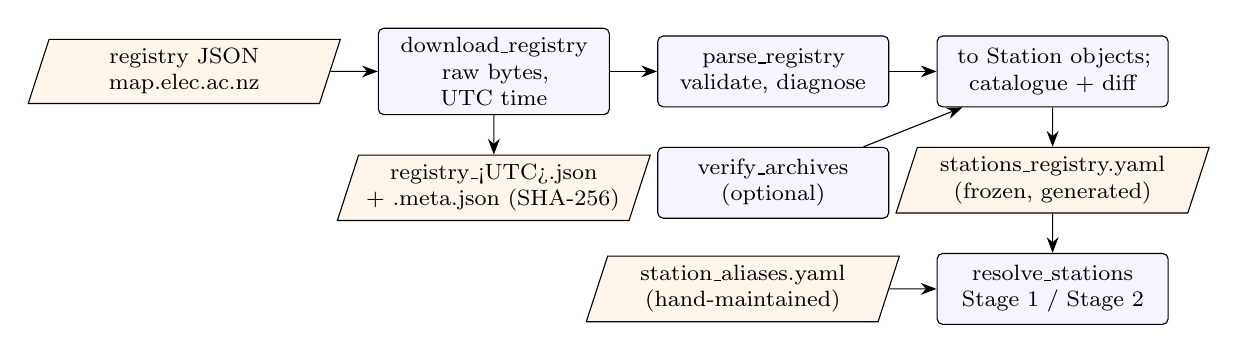
\begin{tikzpicture}[node distance=5mm and 6mm,
  box/.style={draw,rounded corners=2pt,fill=blue!4,align=center,font=\footnotesize,minimum height=9mm,text width=27mm},
  io/.style={draw,trapezium,trapezium left angle=72,trapezium right angle=108,fill=orange!8,align=center,font=\footnotesize,text width=32mm},
  >={Stealth[length=2mm]}]
\node[io] (api) {registry JSON\\map.elec.ac.nz};
\node[box, right=of api] (fetch) {download\_registry\\raw bytes, UTC time};
\node[box, right=of fetch] (parse) {parse\_registry\\validate, diagnose};
\node[box, right=of parse] (conv) {to Station objects;\\catalogue + diff};
\node[io, below=of fetch] (snap) {registry\_<UTC>.json\\+ .meta.json (SHA-256)};
\node[box, below=of parse] (arch) {verify\_archives\\(optional)};
\node[io, below=of conv] (cat) {stations\_registry.yaml\\(frozen, generated)};
\node[box, below=of cat] (res) {resolve\_stations\\Stage 1 / Stage 2};
\node[io, left=of res] (al) {station\_aliases.yaml\\(hand-maintained)};
\draw[->] (api) -- (fetch); \draw[->] (fetch) -- (parse); \draw[->] (parse) -- (conv);
\draw[->] (fetch) -- (snap); \draw[->] (arch) -- (conv);
\draw[->] (conv) -- (cat); \draw[->] (cat) -- (res); \draw[->] (al) -- (res);
\end{tikzpicture}
\caption{Station-registry data flow. Only \code{download\_registry} and the
optional archive check use the network. Stage~1 and Stage~2 read the frozen
catalogue.}
\label{fig:registry}
\end{figure}

\section{Retrieval, snapshots and normalisation}

\paragraph{Retrieval.} \code{tart\_gnss.registry} is the only module that
contacts the registry or knows its JSON layout. It never scrapes the map
HTML. The response is kept as raw bytes, and each successful refresh writes
\code{data/stations/registry\_<UTC>.json} (the exact payload),
a sidecar \code{registry\_<UTC>.meta.json} (source URL, retrieval time,
SHA-256, station count) and \code{latest.json}. Historical snapshots are
never overwritten. If the registry cannot be reached, returns an HTTP error
or returns invalid JSON, a \code{RegistryFetchError} is raised and no file is
changed. The registry embeds ``last seen'' timestamps, so the snapshot hash
changes on every fetch even when no station has changed; changes are
therefore assessed with the catalogue diff described below, not the hash.

\paragraph{Parsing.} The supported schema is a mapping with a
\code{telescopes} list, whose entries carry \code{nodeName},
\code{telescopeName} and \code{telescopeInfo.info.location}
$\{$\code{lat}, \code{lon}, \code{alt}$\}$. Any other top-level structure raises
\code{RegistrySchemaError}. Each entry is validated with the same
\code{validate\_coordinates} function used for hand-written catalogues
(finite numbers; latitude in $[-90,90]$; longitude in $[-180,180]$; height
in $[-500,9000]$\,m). A malformed entry is skipped and recorded as a
diagnostic, and a missing value is never replaced by zero. If two entries
share a TART id, the registry is ambiguous about that station, so every
copy is skipped. With \code{--strict}, any such entry raises
\code{RegistryStationError}.

\paragraph{Derived metadata.} The registry does not publish API URLs or
archive locations. \code{api\_url} is derived from the convention
\code{https://api.elec.ac.nz/tart/<tart\_id>} in a single function,
\code{default\_api\_url}. It is recorded as convention-derived and does not
mean that the API is online. Registry presence also does not imply archived
data. \code{archive\_name} is set only when \code{--verify-archives} finds
at least one object under \code{<tart\_id>/vis/} in the archive bucket
(Section~\ref{sec:archive}). In that case \code{archive\_verified} and
\code{archive\_verified\_utc} record the check. Verifications are carried
over from the previous catalogue, and a failed query never erases one.

\paragraph{Catalogue.} The result is written to
\code{stations\_registry.yaml}, a generated file keyed by TART id. Its
\code{metadata} block records the source URL, retrieval time, snapshot
SHA-256 and file name, the number of registry entries and valid stations,
the skipped entries with reasons, and the changes from the previous
catalogue. Each station's \code{source} field names the registry, node,
retrieval time and snapshot hash. The catalogue is read by the existing
\code{load\_stations}. The original alias-keyed \code{stations.yaml} remains
a supported legacy catalogue with the same format.

\section{Identifier resolution}

\code{resolve\_stations} tries each requested identifier, in order, as (1)
an exact catalogue id, (2) a normalised id (case-insensitive, with
\code{-} equivalent to \code{\_}), (3) an alias, whose target is then
resolved by id or TART id, and (4) a station's TART id. Thus
\code{za-rhodes}, \code{za\_rhodes} and \code{south\_africa} all select the
same station, and requesting the same station twice (for example
\code{mauritius mu-udm}) is rejected. An unknown name, or an alias that
points outside the catalogue, fails with a message listing the known
stations and aliases.

\section{Change detection}

Every refresh is compared with the previous catalogue, matching stations by
TART id. New and removed stations, display-name changes, metadata changes
(\code{api\_url}, \code{archive\_name}, \code{archive\_verified}) and
coordinate changes are reported. A coordinate change is reported with its
latitude, longitude and height deltas and with the straight-line
displacement
\begin{equation}
\Delta = \lVert \vect r(\phi',\lambda',h') - \vect r(\phi,\lambda,h)\rVert,
\end{equation}
where $\vect r$ is the Earth-centred Cartesian position from Skyfield's
WGS84 model, so horizontal and vertical changes both contribute. A
displacement above a configurable flag level (\SI{100}{\metre} by default)
is logged as a warning. This level is only a reporting threshold, chosen to
be well above the metre-level rounding seen in the registry. No change is
rejected on this basis. The change record is written next to the snapshot
(\code{registry\_<UTC>.diff.json}) and into the catalogue metadata.

\section{Command-line tools}

\begin{lstlisting}
tart-stations-list                         # packaged catalogue, with aliases
tart-stations-list --archive-only --format json
tart-stations-update                       # snapshot + data/stations/stations_registry.yaml
tart-stations-update --verify-archives     # also check <tart_id>/vis/ in the archive
tart-stations-update --diff --dry-run      # report changes, write nothing
tart-stations-update --verify-archives \
    --output src/tart_gnss/config/stations_registry.yaml   # refresh the packaged default
\end{lstlisting}
Further options of \code{tart-stations-update} are \code{--registry-url},
\code{--snapshot-dir}, \code{--strict}, \code{--timeout},
\code{--displacement-warning-m} and \code{--aliases}, which warns about
aliases whose target has disappeared. The command exits with status~1 if the registry
cannot be retrieved, and the message names the frozen catalogue that
remains available.

\section{Reproducibility rules}

\begin{itemize}
\item \code{tart-common-gnss} reads the packaged frozen catalogue by default and
needs no network access. A live refresh happens only with
\code{--refresh-stations}, which writes a run-specific catalogue and
snapshot under \code{data/stations/}.
\item Stage-1 run metadata copy the selected stations' full coordinates and
record \code{station\_catalogue\_path}, \code{station\_file\_sha256},
\code{station\_registry\_source}, \code{station\_registry\_retrieved\_utc},
\code{station\_registry\_sha256} and the alias file. Results and metadata
carry \code{schema\_version}~2, in which stations are identified by TART id.
Older, unversioned files identify them by legacy names such as
\code{mauritius} and remain readable.
\item Stage~2 never refreshes stations. It takes each station's identity and
coordinates from the Stage-1 results, and uses the catalogue only for
archive and API metadata (Section~\ref{sec:stage2method}). If the catalogue
coordinates now differ, the manifest records
\code{station\_metadata\_changed: true} together with the catalogue values.
\end{itemize}

\section{Current network}

The packaged catalogue was generated from the registry retrieved on
2026-10-09 at 16:06:41~UTC (snapshot SHA-256 \code{df55cafb\dots}). Of 18
entries, 17 validated. \code{bw-biust} was skipped because it publishes no
height, and its latitude and longitude are those of New York, a placeholder.
The archive prefix was verified for 14 stations. No archive data were found
for \code{nz-test}, \code{nz-rock2f} and \code{tart3-test}. The seven
stations of the previous hand-maintained file have identical coordinates in
the registry. Only their display names differ, and they gained explicit
archive verifications. Table~\ref{tab:network} lists the valid stations.

\begin{table}[h]
\centering
\caption{Valid stations of the packaged registry catalogue (WGS84, as
published; height datum undocumented). Alt.\ in metres. ``Archive'' marks a
verified \code{<tart\_id>/vis/} prefix.}
\label{tab:network}
\footnotesize
\setlength{\tabcolsep}{3.5pt}
\begin{tabular}{l>{\raggedright\arraybackslash}p{2.3cm}>{\raggedright\arraybackslash}p{3.3cm}rrrc}
\toprule
TART id & Alias & Display name & Lat.\ (deg) & Lon.\ (deg) & Alt. & Archive\\
\midrule
\code{bd-iub} & -- & IUB - Bangladesh & $23.815474$ & $90.427748$ & 50 & \checkmark\\
\code{ghana} & \code{ghana} & GRAO - Ghana & $5.749725$ & $-0.305557$ & 72 & \checkmark\\
\code{it-ant} & -- & Italia - Antola & $44.591152$ & $9.203245$ & 1400 & \checkmark\\
\code{mg-tana} & \code{madagascar} & Madagascar - Antananarivo & $-18.8971446$ & $47.5551677$ & 1280 & \checkmark\\
\code{mu-udm} & \code{mauritius} & Bel Air - Mauritius & $-20.2587508$ & $57.7591989$ & 20 & \checkmark\\
\code{na-unam} & \code{namibia} & Namibia - UNAM & $-22.612053$ & $17.856784$ & 1655 & \checkmark\\
\code{nz-dunedin} & -- & Dunedin - Testbench & $-45.8568084^\dagger$ & $170.5291560^\dagger$ & 110 & \checkmark\\
\code{nz-elec} & -- & New Zealand - Dunedin & $-45.85177$ & $170.5456$ & 270 & \checkmark\\
\code{nz-nelson} & -- & Nelson - New Zealand & $-41.277584$ & $173.271655$ & 26 & \checkmark\\
\code{nz-nelson-32} & -- & Nelson & $-41.277584$ & $173.271655$ & 26 & \checkmark\\
\code{nz-rock2f} & -- & New Zealand - Rock Test Dunedin & $-45.85177$ & $170.5456$ & 270 & --\\
\code{nz-test} & -- & NZ Test TART: Dunedin & $-45.85177$ & $170.5456$ & 270 & --\\
\code{se-kth} & -- & Sweden - KTH & $59.349$ & $18.07$ & 28 & \checkmark\\
\code{tart3-test} & -- & TUK/KSA - Kenya & $-1.2921912$ & $36.8255432$ & 751 & --\\
\code{za-hammanskraal} & \code{south\_africa\_hammanskraal} & Kwalata - South Africa & $-25.38948$ & $28.32231$ & 1163 & \checkmark\\
\code{za-rhodes} & \code{south\_africa} & Rhodes University, Grahamstown & $-33.319413$ & $26.507688$ & 642.26 & \checkmark\\
\code{zm-cbu} & \code{zambia} & Copperbelt University - Zambia & $-12.80527778$ & $28.23722222$ & 1270 & \checkmark\\
\bottomrule
\end{tabular}

\smallskip
{\footnotesize $^\dagger$ rounded here to 7 decimals; the catalogue keeps the registry's full precision.}
\end{table}

Several entries share a site. For example, \code{nz-elec}, \code{nz-test}
and \code{nz-rock2f} have identical coordinates, as do \code{nz-nelson} and
\code{nz-nelson-32}. They are distinct registered telescopes and are kept
as such. Choosing among them is a scientific decision, not a registry one.

\section{Registry verification}

There are 36 registry tests. They use local registry fixtures and mocked
HTTP, so none of them needs the network:
\begin{itemize}
\item a valid registry normalises every entry; \code{null}, absent,
non-finite or non-numeric coordinates are skipped and never become zero;
a longitude above \ang{180} is rejected by the shared validator; missing
locations and ids are diagnosed; strict mode raises;
\item duplicated TART ids are diagnosed and excluded, and raise in strict
mode; unexpected top-level structures raise \code{RegistrySchemaError};
\item conversion keeps the TART id, the provenance and the
convention-derived API URL; \code{archive\_name} is set only after a
successful verification; a failed archive query leaves the station
unverified without erasing an earlier verification;
\item a catalogue written to disk reloads into identical \code{Station}
objects and exposes its metadata;
\item aliases and TART ids resolve to the same station; mixed duplicates
and unknown aliases fail clearly; the bundled aliases resolve in the
bundled catalogue; the legacy file still resolves by name and TART id;
\item SHA-256 is deterministic, the snapshot and sidecar are written as
specified, and an existing snapshot is never overwritten;
\item the diff detects an added station, a removed station, a coordinate
change (\SI{0.001}{\degree} of latitude at \ang{33}\,S gives
$\approx$\SI{111}{\metre}), a name change and metadata changes;
\item a timeout, an HTTP 502 or a non-JSON response leaves the existing
catalogue untouched and creates no snapshot directory; an end-to-end
refresh writes the snapshots, catalogue and change record; a dry run writes
nothing; \code{tart-stations-list} prints aliases and filters by archive.
\end{itemize}
Further tests check that the packaged and legacy catalogues have identical
coordinates for their shared stations, and that Stage~2 resolves legacy
Stage-1 identifiers through aliases and uses the Stage-1 coordinates when
the catalogue has changed.

%======================================================================
\part{Stage 1: common GNSS visibility windows}
%======================================================================

%======================================================================
\section{Problem definition}
%======================================================================

For satellite $s$, station $i$ and UTC time $t$, let $E_{s,i}(t)$ be the
geometric (unrefracted) topocentric elevation above the WGS84 local
horizontal. Satellite $s$ is visible from station $i$ when
\begin{equation}
E_{s,i}(t) \ge E_{\min}, \qquad E_{\min} = \ang{20}\ \text{(default)}.
\end{equation}
For a set of stations $\mathcal{S}$ (three in Stage~1) simultaneous
visibility is
\begin{equation}
V_s(t) = \bigwedge_{i\in\mathcal{S}} \bigl[E_{s,i}(t)\ge E_{\min}\bigr]
\;\Longleftrightarrow\; \min_{i\in\mathcal{S}} E_{s,i}(t) \ge E_{\min}.
\label{eq:common}
\end{equation}
A \emph{common visibility window} is a maximal continuous interval
$[t_{\rm start},t_{\rm end}]$ on which $V_s(t)$ is true, with duration
$T_{\rm common}=t_{\rm end}-t_{\rm start}$. Every window is kept as a separate
record (a satellite may have several per day), and the primary result is the
list of satellite/window pairs ranked by decreasing $T_{\rm common}$.

%======================================================================
\section{Input data and provenance}
%======================================================================

\subsection{Station coordinates}

Station coordinates are never written into the code. By default they are
read from the frozen registry catalogue \code{stations\_registry.yaml}
(Part~\ref{sec:registry-part}). Any YAML or JSON catalogue in the same format
can be given with \code{--station-file}, including the legacy hand-maintained
\code{stations.yaml}. Each entry records the WGS84 geodetic latitude,
longitude and height, the TART telescope identifier, its REST API URL, and
the provenance of the coordinates. No coordinate was estimated or invented.
All values come from the TART network registry
(\url{https://map.elec.ac.nz/api/v1/telescopes}, field
\code{telescopeInfo.info.location}), which mirrors each telescope's own
\code{/api/v1/info} endpoint. For \code{za-rhodes} the values were
independently confirmed from
\url{https://api.elec.ac.nz/tart/za-rhodes/api/v1/info}. The Stage-1
results in this report were produced on 2026-10-07 from the legacy file
(registry retrieved at 10:03~UTC that day). They therefore identify
stations by legacy names such as \code{mauritius}. The registry snapshot of
2026-10-09 gives identical coordinates. Table~\ref{tab:stations} lists the
three stations used in this report. Any other registered station
(Table~\ref{tab:network}) can be used without code changes.

\begin{table}[h]
\centering
\caption{Stations of the Stage-1 triplet. Coordinates as published by TART
(WGS84; height datum undocumented by the source). ITRS vectors computed by
Skyfield.}
\label{tab:stations}
\small
\begin{tabular}{llrrrr}
\toprule
Legacy ID & TART id & Lat.\ (deg) & Lon.\ (deg) & Alt.\ (m) & ITRS $(x,y,z)$ (km)\\
\midrule
\code{mauritius}    & \code{mu-udm}    & $-20.2587508$ & $57.7591989$ & 20.00   & (3193.40, 5063.04, $-2194.60$)\\
\code{madagascar}   & \code{mg-tana}   & $-18.8971446$ & $47.5551677$ & 1280.00 & (4074.72, 4455.38, $-2053.00$)\\
\code{south\_africa} & \code{za-rhodes} & $-33.319413$  & $26.507688$  & 642.26  & (4774.72, 2381.39, $-3483.97$)\\
\bottomrule
\end{tabular}
\end{table}

Two caveats apply. (i) These are the coordinates configured on each
telescope by its operators; their survey accuracy is not documented. An
error of a few metres is irrelevant for visibility prediction but will matter
for the Stage-5 inference, where surveyed antenna-array centres should be
used. (ii) The alias \code{south\_africa} denotes the Rhodes University
telescope; South Africa also hosts \code{za-hammanskraal}, with the alias
\code{south\_africa\_hammanskraal}. Configuration loading validates each
coordinate (latitude in $[-90,90]$, longitude in $[-180,180]$, height in
$[-500,9000]$\,m, finite, non-null) and requires a non-empty \code{source}.

\subsection{Satellite catalogue}

Orbits are described by TLEs. When no catalogue is supplied the software
downloads the CelesTrak GP groups \code{gps-ops}, \code{galileo},
\code{beidou} and \code{glo-ops} \cite{celestrak}. The combined file is
archived as \code{data/tle/gnss\_<retrieval time>.tle}, never overwritten,
together with a sidecar \code{.meta.json} that records the source URLs, the
retrieval time, the SHA-256 hash of the file and the constellation of each
NORAD ID (taken from the CelesTrak group, not guessed from the name). On
reload, a SHA-256 mismatch between file and sidecar is a hard error. When a
user-supplied file has no sidecar, constellations are inferred from
satellite names with conservative patterns (\code{COSMOS} names are labelled
GLONASS only in the CelesTrak \code{COSMOS~nnnn~(slot)} form); unmatched
satellites are labelled \code{UNKNOWN} and reported. Every TLE line is checked
for length, modulo-10 checksum and NORAD-ID consistency.

For each satellite the software keeps the constellation, name, NORAD ID, TLE
lines and epoch, and for each window the signed TLE age
$\Delta t_{\rm TLE}=t_{\rm obs}-t_{\rm epoch}$ at the window start, middle
and end (negative values mean the elements are propagated backwards).

\subsection{TLE age diagnostics}

SGP4 accuracy degrades with $|\Delta t_{\rm TLE}|$, at a rate that depends on
the orbit and on the quality of the element set; there is no universal
threshold. The software therefore (a) stores $\Delta t_{\rm TLE}$ for every
window, (b) warns whenever any epoch of the search interval precedes the TLE
epoch --- the typical symptom of using a modern catalogue to reconstruct an
older observation --- and (c) warns when $|\Delta t_{\rm TLE}|$ exceeds a
user-configurable flag level (\code{--tle-age-warning-days}, default 3~days).
The flag level is a project convention, not an accuracy bound. For
historical observations, a catalogue contemporaneous with the observation
(for instance from Space-Track) should be supplied with \code{--tle-file}.

%======================================================================
\section{Method}
%======================================================================

\subsection{Time}

All times are UTC. Command-line times are ISO-8601; an explicit \code{Z} or
offset is honoured and converted to UTC, and a timezone-naive value is, by
documented convention, interpreted as UTC (and logged as such). Internally,
sample epochs are elapsed SI seconds from the start time, added on the TT
scale by Skyfield, so leap seconds are handled correctly. Skyfield's
built-in leap-second and $\Delta T$ tables are used so that runs need no
network access beyond the TLE download and are reproducible for a given
Skyfield version.

\subsection{Orbit propagation and topocentric geometry}

Propagation uses the SGP4 implementation of the \code{sgp4} package through
Skyfield \cite{skyfield,sgp4,vallado2006}; no orbital mechanics or frame
transformation is implemented by hand. For a station at geodetic position
$(\phi_i,\lambda_i,h_i)$ the vector difference
\code{(satellite - station).at(t)} gives the geometric topocentric position,
from which Skyfield returns azimuth $A_i$ (from north through east),
elevation $E_i$, range $\rho_i$ and range rate $\dot\rho_i$. Light-time,
aberration and refraction are not applied: the quantities describe geometric
lines of sight, which is what the Stage-5 forward model needs. (At
$E=\ang{20}$ tropospheric refraction raises the apparent elevation by about
$\ang{;2.7;}$, irrelevant to visibility but to be considered when comparing with
measured TART directions.)

\subsection{Earth-fixed satellite positions}

For each window the satellite position $\vect r_s$ and velocity are computed
at the start, midpoint and end in the International Terrestrial Reference
System (ITRS) using Skyfield's \code{frame\_xyz\_and\_velocity(itrs)}, which
converts SGP4's TEME output via the Earth's rotation, precession and
nutation. Skyfield's ITRS neglects polar motion unless polar-motion tables
are loaded, an approximation at the $\sim$\SI{10}{\metre} level. The
station positions $\vect r_i$ are expressed in the same frame from their
WGS84 coordinates. The geometric line of sight and its unit vector,
\begin{equation}
\vect d_i = \vect r_s - \vect r_i, \qquad
\hat{\vect d}_i = \vect d_i / \lVert \vect d_i \rVert ,
\end{equation}
are stored at the window midpoint for every station. All Cartesian outputs
carry the label \code{coordinate\_frame = "ITRS"}.

\subsection{Coarse sampling and boundary refinement}

Each satellite is propagated on a uniform grid with step $\Delta$
(default \SI{10}{\second}) that always includes both ends of the interval.
The boolean series $V_s(t_k)$ of Eq.~\eqref{eq:common} is split into maximal
runs of \code{True}. A run starting at sample $k$ brackets a rise between
$t_{k-1}$ (false) and $t_k$ (true); this bracket is refined by bisection on
the exact predicate $V_s(t)$ until it is narrower than a tolerance $\tau$
(default \SI{0.1}{\second}, i.e.\ $\lceil\log_2(\Delta/\tau)\rceil = 7$
iterations). The reported boundary is the \code{True}-side end of the final
bracket, so it is always inside the original bracket, satisfies $V_s=$ true,
and is within $\tau$ of the true crossing. Setting boundaries are treated
symmetrically. Runs touching the edges of the search interval are not
refined and are flagged as \emph{clipped} (the real window may be longer).

Because the predicate is the minimum elevation over stations, the window
boundaries are determined by whichever station is limiting at that moment;
in the results the limiting station shows $E=\ang{20.0000}$ at the boundary
(Section~\ref{sec:verification}). The only geometric limitation of the
approach is that excursions shorter than $\Delta$ (a satellite briefly
dipping below or rising above the threshold between two samples) cannot be
detected; for GNSS orbits, whose elevations change by roughly a tenth of
a degree or less per \SI{10}{\second}, this is not a practical concern, and $\Delta$
can be reduced if needed.

\subsection{Ranking}

Windows shorter than \code{--min-duration} are discarded. The remainder are
sorted by decreasing duration, ties broken by start time and then NORAD ID,
giving a deterministic 1-based rank.

%======================================================================
\section{Software}
%======================================================================

\subsection{Architecture}

The package \code{tart\_gnss} (Python $\ge 3.9$; dependencies NumPy,
Skyfield, sgp4, PyYAML, requests) is organised as in Table~\ref{tab:modules} and
Fig.~\ref{fig:flow}. Visibility and window logic operate on a sequence of
stations of any length; only the CLI enforces the Stage-1 requirement of
exactly three stations. Network access is confined to the TLE module and,
when explicitly requested, the registry module.
Diagnostics use Python's \code{logging} with UTC timestamps; only the final
summary is printed.

\begin{table}[h]
\centering
\caption{Package modules.}
\label{tab:modules}
\small
\begin{tabular}{lp{11cm}}
\toprule
Module & Responsibility\\
\midrule
\code{stations.py} & load YAML/JSON catalogues and aliases; validate coordinates; resolve identifiers (id, normalised id, alias, TART id)\\
\code{registry.py} & TART registry: download, snapshots with SHA-256, schema-checked parsing, archive verification, catalogue generation, diffs\\
\code{registry\_cli.py} & \code{tart-stations-update} and \code{tart-stations-list}\\
\code{tle.py} & parse and checksum TLEs; epochs; constellation labels; CelesTrak download and archival with SHA-256 sidecar\\
\code{propagation.py} & SGP4 via Skyfield; azimuth, elevation, range, range rate; ITRS positions; line-of-sight vectors\\
\code{visibility.py} & $E_i\ge E_{\min}$ per station and the AND over $N$ stations; exact predicate for refinement\\
\code{windows.py} & runs of \code{True}; bisection refinement; \code{Window} objects with clipping flags\\
\code{search.py} & orchestration over satellites; window characterisation; TLE-age diagnostics\\
\code{output.py} & ranking; CSV; detailed JSON; terminal summary\\
\code{provenance.py} & software versions, hashes and run metadata\\
\code{cli.py} & argument parsing, validation, logging, file naming\\
\bottomrule
\end{tabular}
\end{table}

\begin{figure}[h]
\centering
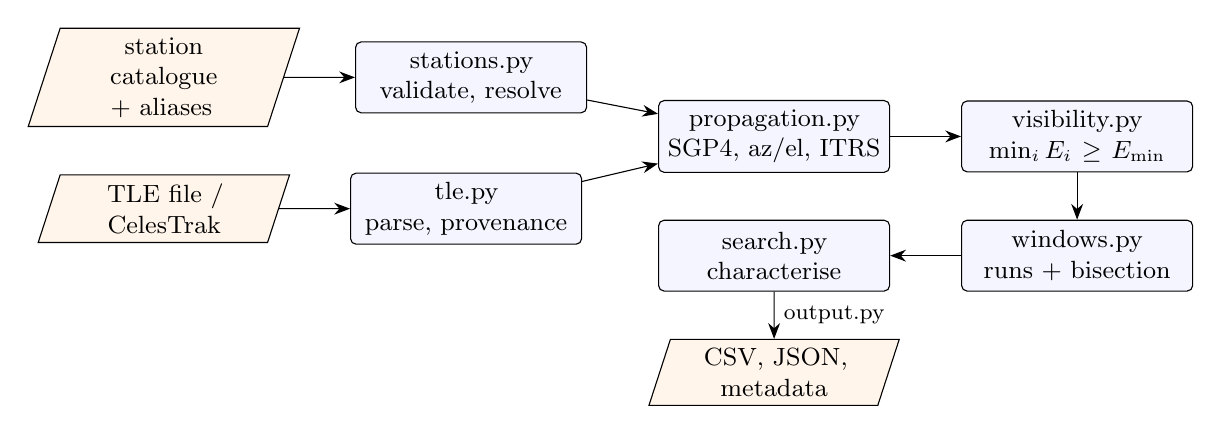
\begin{tikzpicture}[node distance=6mm and 9mm,
  box/.style={draw,rounded corners=2pt,fill=blue!4,align=center,font=\small,minimum height=9mm,text width=27mm},
  io/.style={draw,trapezium,trapezium left angle=72,trapezium right angle=108,fill=orange!8,align=center,font=\small,text width=24mm},
  >={Stealth[length=2mm]}]
\node[io] (st) {station catalogue\\+ aliases};
\node[io, below=of st] (tle) {TLE file /\\CelesTrak};
\node[box, right=of st] (ld) {stations.py\\validate, resolve};
\node[box, right=of tle] (tl) {tle.py\\parse, provenance};
\node[box, right=of ld, yshift=-7.5mm] (pr) {propagation.py\\SGP4, az/el, ITRS};
\node[box, right=of pr] (vi) {visibility.py\\$\min_i E_i \ge E_{\min}$};
\node[box, below=of vi] (wi) {windows.py\\runs + bisection};
\node[box, left=of wi] (se) {search.py\\characterise};
\node[io, below=of se] (out) {CSV, JSON,\\metadata};
\draw[->] (st) -- (ld); \draw[->] (tle) -- (tl);
\draw[->] (ld) -- (pr); \draw[->] (tl) -- (pr);
\draw[->] (pr) -- (vi); \draw[->] (vi) -- (wi);
\draw[->] (wi) -- (se); \draw[->] (se) -- node[right,font=\footnotesize]{output.py} (out);
\end{tikzpicture}
\caption{Data flow of a Stage-1 run.}
\label{fig:flow}
\end{figure}

\subsection{Installation and use}

\begin{lstlisting}
pip install .                      # or: pip install -e ".[dev]"
tart-common-gnss --stations mauritius madagascar south_africa \
    --start 2026-10-01T00:00:00Z --end 2026-10-02T00:00:00Z \
    --min-elevation 20 --step 10
\end{lstlisting}
\code{python common\_gnss.py} and \code{python -m tart\_gnss} are equivalent.
Stations may be given as TART ids (\code{mu-udm mg-tana za-rhodes}) or as
aliases; both select the same stations. Optional arguments:
\code{--tle-file} (use an archived catalogue exactly), \code{--tle-dir},
\code{--constellations GPS Galileo \dots}, \code{--output},
\code{--station-file}, \code{--aliases}, \code{--refresh-stations} (fetch
the live registry first; off by default), \code{--station-snapshot-dir},
\code{--min-duration},
\code{--tolerance}, \code{--tle-age-warning-days}, \code{--verbose}. Input
errors (unknown station, malformed date, start not before end, wrong number
of stations) terminate with exit status~2 and a clear message.

\subsection{Outputs}

A run writes three files (default \code{results/\allowbreak common\_gnss\_YYYYMMDD.csv},
\code{.json} and \code{run\_metadata\_YYYYMMDD.json}):
\begin{description}
\item[CSV] one row per satellite$\times$window: rank, satellite, NORAD ID,
constellation, start/end (UTC), duration, clipping flags, threshold; for each
station its identifier and azimuth/elevation at start, middle and end plus
the mid-window range; midpoint ITRS satellite position with the frame name;
TLE epoch, TLE age at start and middle, TLE source. TLE lines are not
embedded in the CSV.
\item[JSON] \code{schema\_version}; run parameters; frame description; stations with ITRS vectors
and sources; catalogue provenance; every searched satellite with full TLE;
and for every window the station geometry (azimuth, elevation, range, range
rate) at start/mid/end, satellite ITRS position and velocity at the same
epochs, midpoint line-of-sight vectors, and the TLE lines, epoch and ages.
\item[Metadata] versions of \code{tart\_gnss}, Python, Skyfield, sgp4, NumPy
and PyYAML; platform; run timestamp; full command line; interval;
stations and coordinates; the station catalogue path and SHA-256; the
registry source, retrieval time and snapshot SHA-256; threshold, step and
tolerance; TLE file, source, retrieval time and SHA-256; TLE-age summary;
failed propagations; output paths.
\end{description}

%======================================================================
\section{Stage-1 verification}
\label{sec:verification}
%======================================================================

The Stage-1 tests (\code{pytest}, 64 tests, $<\SI{1}{\second}$) cover:
\begin{itemize}
\item \textbf{Stations:} latitude \ang{100}, longitude \ang{300}, implausible
heights, \code{null} or non-numeric coordinates and missing provenance are
rejected; unknown and duplicated stations fail with clear messages; the
bundled registry catalogue and the legacy file validate, are sourced, and
agree on every shared station.
\item \textbf{TLEs:} checksum, two- and three-line parsing, epoch decoding,
name classification, constellation filtering, archival with sidecar
metadata (network mocked) and detection of a modified catalogue.
\item \textbf{Visibility:} the synthetic example
$A=[19,21,25,18]$, $B=[22,23,24,25]$, $C=[30,30,19,30]$ with $E_{\min}=\ang{20}$
gives $[\text{F},\text{T},\text{F},\text{F}]$; the threshold is inclusive;
NaN (failed propagation) is not visible; any number of stations works.
\item \textbf{Windows:} \code{F F T T T F} gives one window;
\code{F T T F F T T F} gives two independent windows; refined crossings lie
inside the coarse bracket and within tolerance of an analytic crossing;
clipping flags are set at interval edges.
\item \textbf{Propagation:} orbital radii of real GPS, Galileo, BeiDou-GEO and
GLONASS TLEs match their nominal values; geostationary elevation is nearly
constant; and the Skyfield azimuth/elevation agree to better than
\ang{0.001} with an independent east-north-up projection of the ITRS line of
sight $\vect r_s-\vect r_i$, confirming that the angular and Cartesian outputs
are mutually consistent --- a prerequisite for the Stage-5 forward model.
\item \textbf{CLI:} start after end, malformed dates, unknown stations and
wrong station counts fail clearly; an end-to-end run checks ranking order,
frame labels, TLE lines in the JSON, that every station is above
\ang{20} at window start, middle and end, and that refined boundaries are at
\ang{20} to within \ang{0.01}; a geometry without common visibility reports
``No common GNSS visibility windows found.''
\end{itemize}
In the production run below the limiting station at every refined boundary
has $E=\ang{20.0000}$ (e.g.\ Rhodes at both boundaries of the BeiDou-2~G6
window), and the ITRS radii are \SI{42146}{\kilo\metre} for GEO and
\SI{29594}{\kilo\metre} for Galileo, as expected.

%======================================================================
\section{Stage-1 results: Mauritius--Madagascar--South Africa, 2026-10-01}
%======================================================================

The acceptance run covered 2026-10-01T00:00Z--2026-10-02T00:00Z with
$E_{\min}=\ang{20}$ and $\Delta=\SI{10}{\second}$, using the CelesTrak
catalogue retrieved 2026-10-07T10:11:56Z (145 satellites: 32 GPS, 32
Galileo, 54 BeiDou, 27 GLONASS; SHA-256 \code{1a6c259b\dots f2ea}). The run
took about \SI{6}{\second} of computation (excluding download).

\paragraph{TLE age.} Because the catalogue was retrieved six days after the
observation date, 127 of the 145 satellites have TLE epochs after the start
of the interval and are propagated backwards; the median $|\Delta t_{\rm TLE}|$
is 5.4~days and the maximum 18.3~days. The software warned accordingly. For
window prediction this is adequate, but the results should be regenerated
with a contemporaneous catalogue before they are used as a reference for
Stage~6.

\paragraph{Windows.} 154 common windows were found, involving 135
satellites (Table~\ref{tab:constellations}). Common windows are long because
the three stations are within $\sim$\SI{3200}{\kilo\metre} of each other while
the satellites are at altitudes of 19\,000--36\,000~km. The ten longest are
listed in Table~\ref{tab:top}; the top two are geostationary BeiDou
satellites visible for most or all of the day, so their windows are clipped
by the search interval. Figure~\ref{fig:timeline} shows the forty longest
windows, Fig.~\ref{fig:elevation} the elevation curves of the top-ranked
satellite of each constellation, and Fig.~\ref{fig:sky} the sky tracks of
the top-ranked Galileo satellite as seen from the three stations.

\begin{table}[h]
\centering
\caption{Common windows per constellation (2026-10-01).}
\label{tab:constellations}
\small
\begin{tabular}{lrrrr}
\toprule
Constellation & Satellites searched & Windows & Longest (min) & Median (min)\\
\midrule
GPS     & 32 & 37 & 320.2  & 207.4\\
Galileo & 32 & 32 & 438.2  & 265.7\\
BeiDou  & 54 & 51 & 1440.0$^\ast$ & 267.6\\
GLONASS & 27 & 34 & 264.6  & 188.6\\
\bottomrule
\multicolumn{5}{l}{\footnotesize $^\ast$ geostationary, clipped by the 24-h search interval}
\end{tabular}
\end{table}

\begin{table}[h]
\centering
\caption{Ten longest common windows (UTC, 2026-10-01; $^\ast$ clipped).
$\Delta t_{\rm TLE}$ at window middle.}
\label{tab:top}
\small
\begin{tabular}{rllllrr}
\toprule
Rank & Satellite & NORAD & Start & End & Dur.\ (min) & $\Delta t_{\rm TLE}$ (d)\\
\midrule
1 & BEIDOU-2 G5 (C05)       & 38091 & 00:00:00$^\ast$ & 24:00:00$^\ast$ & 1440.0 & $-5.48$\\
2 & BEIDOU-3 G2 (C60)       & 45344 & 04:07:05 & 24:00:00$^\ast$ & 1192.9 & $-5.39$\\
3 & BEIDOU-2 G6 (C02)       & 38953 & 12:28:02 & 20:16:28 & 468.4 & $-5.29$\\
4 & GSAT0219 (GALILEO 23)   & 43566 & 08:28:07 & 15:46:19 & 438.2 & $-4.86$\\
5 & GSAT0218 (GALILEO 22)   & 43058 & 00:00:00$^\ast$ & 07:11:58 & 432.0 & $-2.53$\\
6 & GSAT0208 (GALILEO 11)   & 41175 & 16:53:47 & 24:00:00$^\ast$ & 426.2 & $-4.27$\\
7 & GSAT0234 (GALILEO 34)   & 67162 & 15:21:34 & 22:24:29 & 422.9 & $-0.78$\\
8 & BEIDOU-2 IGSO-4 (C09)   & 37763 & 16:48:56 & 23:37:48 & 408.9 & $-2.96$\\
9 & GSAT0204 (GALILEO 8)    & 40545 & 07:08:50 & 13:51:50 & 403.0 & $15.64$\\
10 & BEIDOU-3S IGSO-1S (C31) & 40549 & 01:38:59 & 08:08:02 & 389.1 & $-2.80$\\
\bottomrule
\end{tabular}
\end{table}

\begin{figure}[p]
\centering
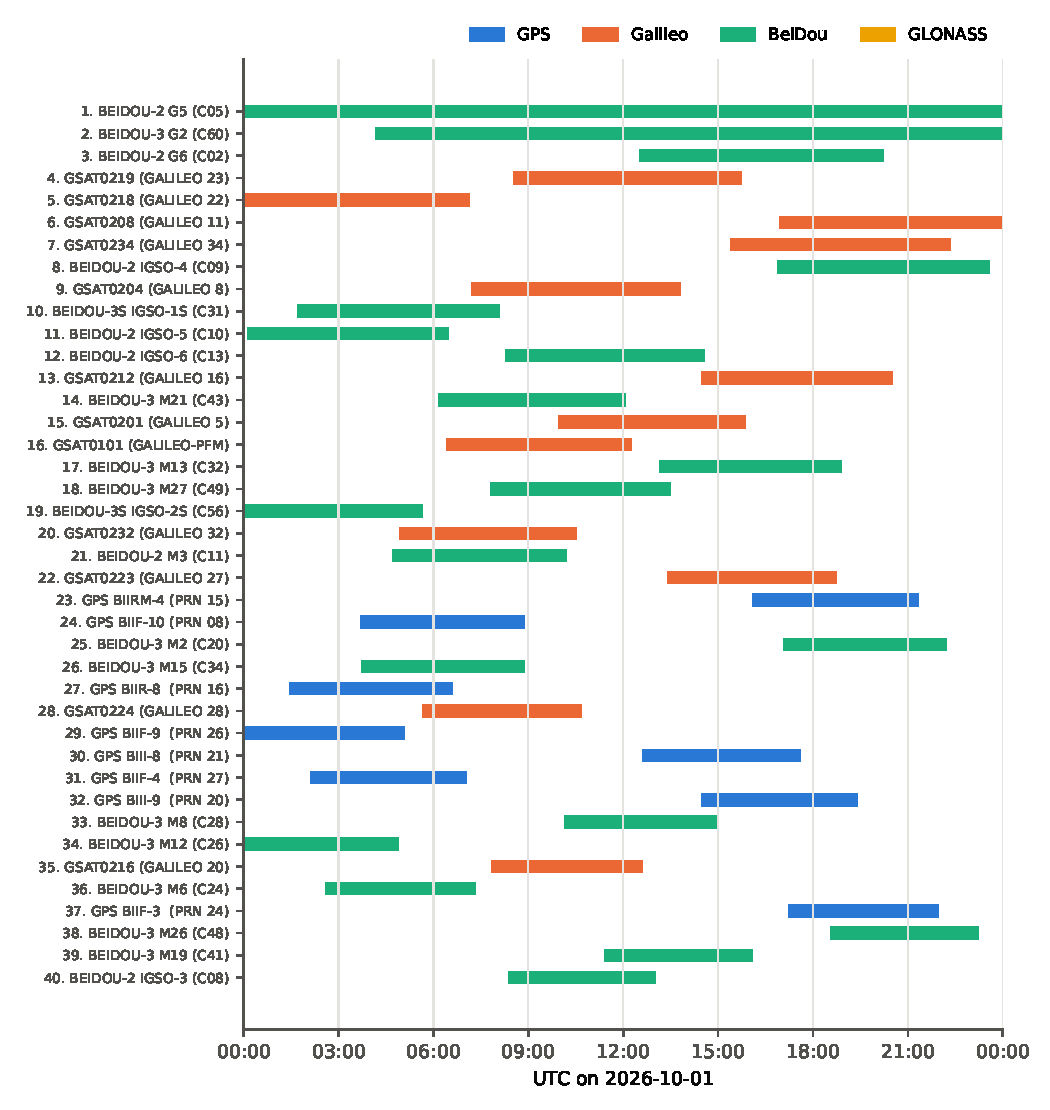
\includegraphics[width=\textwidth]{figures/window_timeline.pdf}
\caption{The forty longest common windows for the Mauritius--Madagascar--South
Africa triplet on 2026-10-01, ordered by rank and coloured by constellation.
Separate windows of the same satellite are separate rows.}
\label{fig:timeline}
\end{figure}

\begin{figure}[p]
\centering
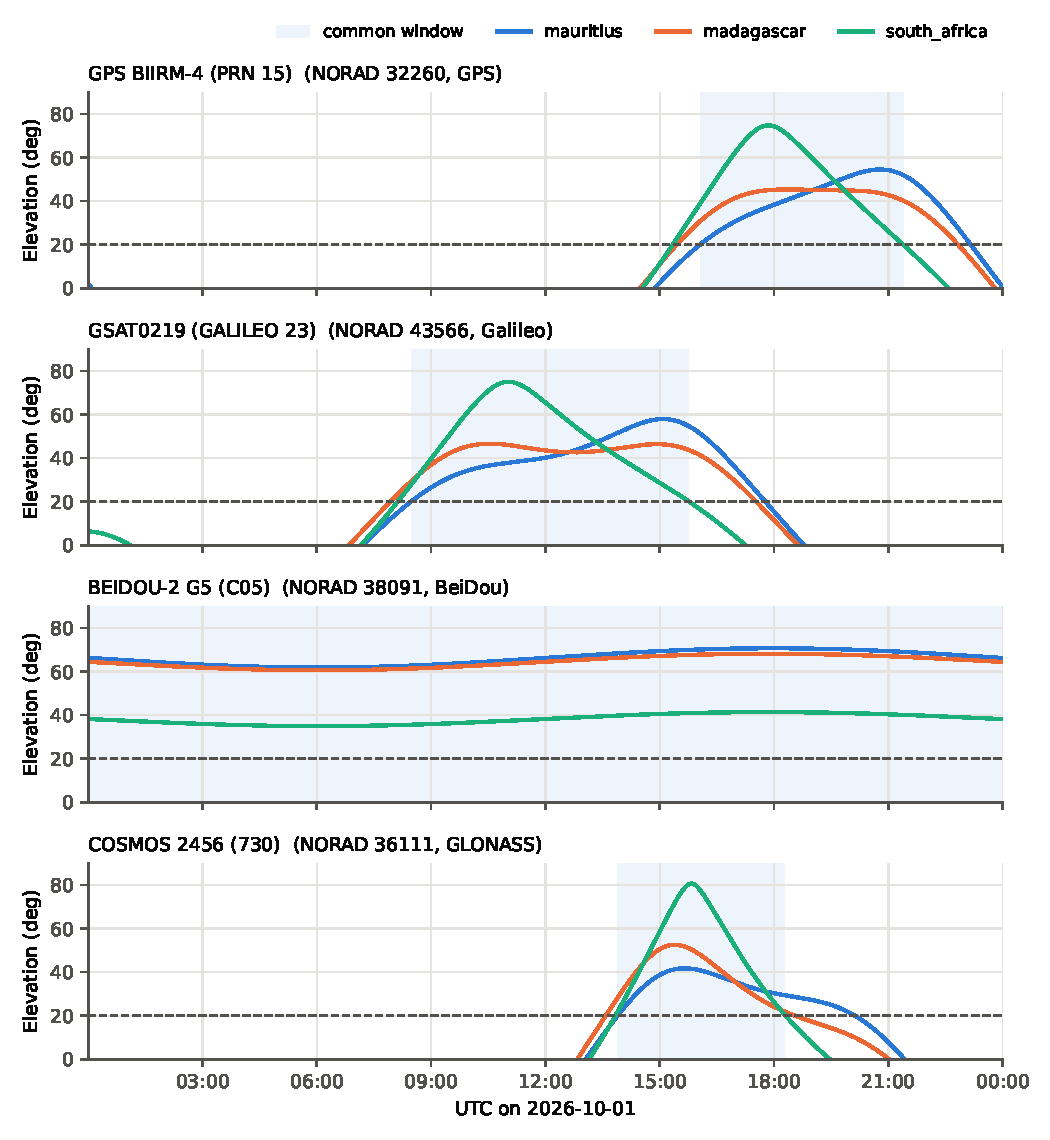
\includegraphics[width=\textwidth]{figures/elevation_examples.pdf}
\caption{Elevation at the three stations for the top-ranked window of each
constellation. The dashed line is $E_{\min}=\ang{20}$; shading marks the
common window, bounded by whichever station is limiting.}
\label{fig:elevation}
\end{figure}

\begin{figure}[h]
\centering
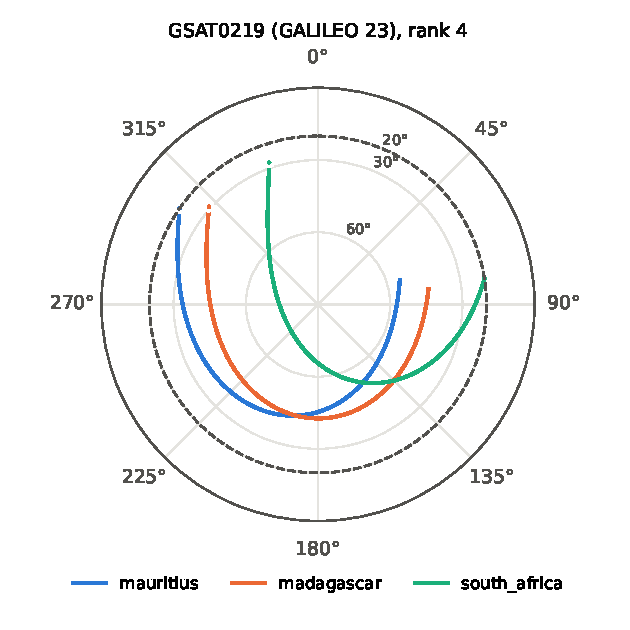
\includegraphics[width=0.55\textwidth]{figures/skyplot.pdf}
\caption{Sky tracks (azimuth clockwise from north, zenith at the centre) of
GSAT0219 during its common window, as seen from each station; dots mark the
window start and the dashed circle the \ang{20} horizon. These are the
directions that TART images will measure in Stages~3--4.}
\label{fig:sky}
\end{figure}

\paragraph{Relevance at 1.575 GHz.} Stage~1 is purely geometric, and
geometric visibility does not imply detectability by TART, which records
\SI{2.5}{\mega\hertz} around \SI{1575.42}{\mega\hertz}. GPS L1, Galileo E1
and BeiDou-3 B1C share this centre frequency, whereas BeiDou-2 transmits B1I
at \SI{1561.098}{\mega\hertz} and the legacy GLONASS L1 FDMA signals lie at
\SIrange{1598}{1606}{\mega\hertz} \cite{gnssbook}. Several of the
top-ranked windows (BeiDou-2 G5, G6, IGSO-4) are therefore unlikely to be
usable. Until signal-level filtering is added, Stage~2 should be driven by
\code{--constellations GPS Galileo} or by BeiDou-3 windows.

%======================================================================
%======================================================================
\part{Stage 2: TART observation retrieval and Measurement-Set preparation}
%======================================================================

\section{Stage-2 objective}
\label{sec:stage2}

Stage~2 takes one Stage-1 window and establishes whether the three TART
stations actually recorded usable visibility data during it. It then
retrieves those data, validates them, measures the real three-station
overlap, and converts each station independently into a CASA Measurement
Set (MS) for Stage-3 imaging. Three conditions are kept strictly separate
throughout:
\begin{description}
\item[geometric visibility] the satellite is above $E_{\min}$ at every
station (Stage~1, from TLEs);
\item[data availability] every station recorded real visibilities covering
a common, non-zero interval (Stage~2, from the native files);
\item[radio detection] the satellite appears in each image (Stage~3).
\end{description}
None of these is inferred from another. In particular, a result is labelled
\emph{three-station valid} only when all three stations hold real, validated
visibility data with a common interval of non-zero length, and, when
conversion was requested, each has a validated MS. Imaging, source
detection, triangulation and inference are not part of Stage~2.

\section{The TART visibility archive}

\subsection{Location and layout}
\label{sec:archive}

The TART project archives native visibility files in a public, read-only S3
bucket. The maintained client \code{tart\_tools.archive\_handler} \cite{tarttools} (used by
\code{tart2ms --archive-search}) defines its location as bucket \code{tart}
at \code{s3.us-west-2.amazonaws.com}, with objects
\begin{center}
\code{<archive\_name>/vis/<year>/<month>/<day>/vis\_<YYYY-MM-DD\_HH\_MM\_SS.ffffff>.hdf},
\end{center}
where month and day are not zero-padded. \code{tart\_gnss} imports this
location from \code{tart\_tools} when it is installed and lists the bucket
with the same \code{minio} client. The archive name of a station equals its
TART identifier (\code{mu-udm}, \code{mg-tana}, \code{za-rhodes}, \dots).
It is stored as \code{archive\_name} in the station catalogue only after
\code{tart-stations-update --verify-archives} has found the prefix in the
bucket (Section~\ref{sec:registry}). On 2026-10-09 this held for 14 of the
17 registered stations. No archive name or URL was guessed.

\subsection{Why the archive helper is not called directly}

\code{tart\_tools.handle\_archive\_request} selects objects by their S3
\code{last\_modified} time. That is the \emph{upload} time, which lags the
observation by minutes; for example, Rhodes data from 00:00:36 were uploaded
at 00:03:24. The helper also renames files to \code{obs\_00000.hdf}, which
discards the archive identifiers needed for provenance. Stage~2 therefore
reuses the archive location and client library but selects files by the
observation time in the filename, and keeps the original names.

\subsection{Native file structure}

Inspection of archive files from \code{za-rhodes}, \code{mg-tana} and
\code{mu-udm} shows a consistent HDF5 layout, which the Stage-2 reader
relies on and validates:
\begin{itemize}
\item \code{config}: a JSON string with \code{name}, \code{frequency}
(\SI{1575.42}{\mega\hertz}), \code{bandwidth} (\SI{2.5}{\mega\hertz}),
\code{lat}/\code{lon}/\code{alt} and \code{num\_antenna} (24);
\item \code{timestamp}: about 60 ISO-8601 UTC timestamps per file, with a
median spacing of \SI{1.025}{\second};
\item \code{vis}: complex visibilities of shape $60\times276$, i.e.\
$24\cdot23/2$ baselines; \code{baselines} and \code{antenna\_positions};
\item \code{gains} and \code{phases}: the per-antenna calibration in use
when the data were recorded; \code{phase\_elaz}: the phase centre.
\end{itemize}
The filename time equals the time of the file's \emph{last} sample, and
consecutive files abut: the next file starts about \SI{1}{\second} later.
A file named $T$ therefore holds data from about $T-\SI{61}{\second}$ to
$T$. Discovery keeps files with $t_{q,\rm start}\le T\le t_{q,\rm end}+m$,
where the margin is $m=\SI{120}{\second}$. Sample times are never taken from
filenames: each retained file is read, and files whose real samples fall
outside the query interval are recorded but not used.

\section{Method}

\subsection{Selection and query interval}
\label{sec:stage2method}

The Stage-1 JSON is loaded, and exactly one window is chosen by
\code{--rank}, or by \code{--norad-id} with \code{--window-index} when the
satellite has several windows. An ambiguous or inconsistent selection is an
error. The window's geometry, TLE and provenance are copied verbatim into
\code{stage1\_window.json} and the manifest, together with the SHA-256 of
the Stage-1 file; Stage-1 geometry is never recomputed. Each Stage-1
station is looked up in the station catalogue by TART id, then by its
Stage-1 id, with aliases accepted. Older results that use names such as
\code{mauritius} therefore still resolve. The catalogue supplies only the
archive name and API URL. Identity and coordinates always come from the
Stage-1 results, and the catalogue is never refreshed during Stage~2. If
the catalogue coordinates differ from the Stage-1 values, a warning is
logged and the manifest records \code{station\_metadata\_changed: true}
with the catalogue coordinates and source next to the Stage-1 values. The
archive query interval is
\begin{equation}
t_{q,\rm start}=t_{\rm pred,start}-P,\qquad t_{q,\rm end}=t_{\rm pred,end}+P,
\end{equation}
with $P=\SI{120}{\second}$ by default. Long windows can be sampled first
with \code{--max-duration}, which keeps only a central portion of the stated
length, centred on the window midpoint, where the elevations are highest.

Each window also receives a \code{signal\_relevance} label. The rules use
only constellation-level facts: \code{GPS\_L1}, \code{GALILEO\_E1},
\code{BEIDOU\_B1C} for BeiDou-3 MEO/IGSO satellites, \code{OUT\_OF\_BAND}
for BeiDou-2 (B1I, \SI{1561.098}{\mega\hertz}), and \code{UNKNOWN}
otherwise (BeiDou-3 GEO, experimental BeiDou-3S, GLONASS). A satellite that
is not in band triggers a warning but is still processed.

\subsection{Retrieval and integrity}

Every file is downloaded under its original name to a temporary
\code{.part} file. Its size and, when the S3 ETag is a plain MD5, its MD5
are checked against the archive listing before it is moved into place. A
sidecar \code{<file>.prov.json} records the remote identifier, URL, size,
ETag, retrieval time and SHA-256. An existing local file is reused only if
its sidecar names the same archive object and its SHA-256 still matches.
Any other existing file stops the run, so nothing is silently overwritten.

\subsection{Native validation}

Each file is opened and checked. Fatal problems exclude the file: the file
is unreadable; timestamps are missing, timezone-naive or not strictly
increasing; the shape of \code{vis} disagrees with the timestamps or
baselines; the visibilities are all zero or non-finite; or the recorded
position is more than \ang{0.01} from the configured station, i.e.\ the data
come from another site. Minor anomalies are recorded as warnings:
non-finite values, an inconsistent antenna count, or missing metadata.
The observing frequency and bandwidth are taken from the file itself. The
data count as in band when \SI{1575.42}{\mega\hertz} lies inside the
recorded band, $|f-\SI{1575.42}{\mega\hertz}|\le B/2$. This tolerance comes
from the instrument metadata and was not chosen independently. Antennas
with zero gain are listed, and a fingerprint of the gain and phase
solutions shows when calibration changes during a window.

\subsection{Temporal coverage and synchronisation}

For each station, all samples are merged into one timeline. The tool reports
the first and last timestamps, the number of samples and the median cadence
$\delta$. A step longer than $3\delta$ is reported as a gap
(\code{--gap-factor}) and splits the timeline into continuous segments
$S_i$. The actual common interval is
\begin{equation}
t_{\rm common,start}=\max_i t_{i,\rm first},\qquad
t_{\rm common,end}=\min_i t_{i,\rm last},
\end{equation}
and it is valid only if $t_{\rm common,end}>t_{\rm common,start}$. Coverage
of the predicted window $W$ is
\begin{equation}
f_i=\frac{T(S_i\cap W)}{T(W)},\qquad
f_{\rm 3\text{-}station}=\frac{T(S_1\cap S_2\cap S_3\cap W)}{T(W)},
\end{equation}
so gaps never count as covered. The same fractions are also reported for
the retrieved part of $W$ when \code{--max-duration} is used. The software
does not assume that the stations' samples are simultaneous. For each
station pair it gives the median and maximum separation between each sample
and the other station's nearest sample, within the common interval.

\subsection{Measurement-Set conversion}

Each station is converted on its own with \code{tart2ms} \cite{tart2ms} (the maintained
TART converter), called with an argument list rather than a shell string:
\begin{center}
\code{tart2ms --hdf <files> --ms <station>.ms --skip-online-source-catalog
--skip-celestial-source-catalog}
\end{center}
The catalogue options are skipped because Stage~2 needs no model data and
should not depend on network access during conversion. Stations are never
concatenated into one interferometer, because they are independent arrays
that will give independent lines of sight. The output must not already
exist. A non-zero exit status, or an MS that is missing, is an error, and
the \code{tart2ms} output is saved to \code{tart2ms.log}. Each MS is then
opened with python-casacore and must have rows, \code{TIME}, \code{UVW} and
\code{DATA} columns, and \code{ANTENNA} and \code{SPECTRAL\_WINDOW} tables,
with the antenna count of the native data. The manifest records the number
of rows, times, antennas and channels, the frequency, the first and last
times, the flagged fraction and the longest baseline.

\paragraph{Calibration.} No calibration algorithm is implemented. By
default \code{tart2ms} applies the \code{gains}/\code{phases} stored in each
native file and flags baselines to antennas whose gain is zero or
non-finite. \code{--uncalibrated} stores the raw visibilities instead. The
manifest records \code{calibration\_status} and \code{calibration\_source}.
It never says the data are calibrated beyond ``solutions applied by
\code{tart2ms} (unverified)''.

\subsection{Manifest and outputs}

A run writes \code{<output>/<YYYYMMDD>/NORAD\_<id>/} containing
\code{stage1\_window.json}, \code{manifest.json}, \code{retrieval.log} and,
for each station, \code{raw/} (native files and \code{.prov.json} sidecars)
and \code{ms/<station>.ms} with \code{tart2ms.log}. The manifest is the
only input Stage~3 needs. It has the sections \code{satellite}, including
\code{signal\_relevance}, the TLE epoch, source and lines; \code{prediction},
covering the predicted and query intervals, padding, the Stage-1 file with
its SHA-256, the ITRS position and lines of sight; \code{stations}, one
entry per station with coordinates, \code{station\_metadata\_changed},
archive status and query bounds, raw
files with hashes, native metadata and coverage, calibration status, the MS
metadata and the Stage-1 predicted az/el; \code{synchronisation};
\code{software}; and \code{provenance}. It is checked against the required
fields before it is written. A previous manifest is renamed
(\code{manifest\_<run tag>.json}), never overwritten. The exit status is 0
for a valid three-station dataset, 3 for a completed run that is not
three-station valid, 2 for invalid input and 1 for failures.
\code{--dry-run} resolves the stations, queries the archives and reports
what would be downloaded without writing anything.

\subsection{Software}

\begin{table}[h]
\centering
\caption{Stage-2 modules (\code{tart\_gnss.stage2}).}
\label{tab:modules2}
\small
\begin{tabular}{l>{\raggedright\arraybackslash}p{10.6cm}}
\toprule
Module & Responsibility\\
\midrule
\code{selection.py} & load the Stage-1 JSON; select one window; query interval; signal relevance\\
\code{archive.py} & archive abstraction (\code{find\_observations}); S3 backend reusing \code{tart\_tools}' archive location\\
\code{download.py} & retrieval; size, MD5/ETag and SHA-256 checks; provenance sidecars; verified reuse\\
\code{native.py} & HDF5 inspection and validation; per-station timeline, cadence and gaps\\
\code{synchronise.py} & common interval; coverage fractions; cross-station timing\\
\code{measurement\_set.py} & \code{tart2ms} wrapper; MS inspection and validation\\
\code{manifest.py} & manifest assembly, schema check and safe writing\\
\code{cli.py} & \code{tart-retrieve}: orchestration, logging, terminal summary\\
\code{errors.py} & \code{Stage1SelectionError}, \code{ArchiveUnavailableError}, \code{ObservationNotFoundError}, \code{DownloadError}, \code{ObservationValidationError}, \code{NoCommonTimeError}, \code{MeasurementSetConversionError}\\
\bottomrule
\end{tabular}
\end{table}

The Stage-2 dependencies are optional extras: \code{pip install
".[stage2]"} installs \code{h5py} and \code{minio}, and \code{".[ms]"}
installs \code{tart2ms} and python-casacore.

\section{Stage-2 verification}

There are 67 Stage-2 tests. They use a mocked archive and synthetic HDF5
files that follow the real layout (random visibilities, not real data), so
they need no live service:
\begin{itemize}
\item selection by valid and invalid rank, a single-window NORAD ID, an
ambiguous NORAD ID, \code{--window-index}, inconsistent rank/NORAD, and
CSV$\to$JSON resolution; signal-relevance rules;
\item padding arithmetic, and the \code{--max-duration} interval centred on
the window midpoint;
\item filename-time parsing; day prefixes across midnight; the file margin;
explicit errors for a missing archive name or an unreachable archive;
\item deterministic SHA-256; provenance sidecars; verified reuse without a
second download; detection of tampered files, unknown files and corrupted
transfers (ETag mismatch);
\item native validation: a valid file, an out-of-band frequency, a wrong
station position, non-monotonic timestamps, missing or all-zero
visibilities, a non-HDF5 file; gap detection across files;
\item the specified temporal intersection (A 10:00--10:20, B 10:03--10:18,
C 10:01--10:25 $\Rightarrow$ 10:03--10:18); no intersection, including
intervals that only touch; coverage fractions; nearest-sample offsets;
\item the \code{tart2ms} wrapper with a mocked runner: success, a
\code{--uncalibrated} run, a non-zero exit, success without an output, an
existing output, an invalid MS and an antenna-count mismatch. A further test
runs the \emph{real} \code{tart2ms} on a synthetic file and is skipped when
\code{tart2ms} is not installed;
\item full CLI runs: a valid three-station run; a missing station, giving
\code{three\_station\_valid=false} with nothing downloaded; partial mode,
which stays invalid; no common time; a query without download; a dry run,
which writes nothing; a conversion failure at one station; a re-run with
verified reuse and the old manifest kept; usage errors; and manifest
validation, including the station count; a changed catalogue coordinate,
which keeps the Stage-1 value and sets \code{station\_metadata\_changed};
and legacy Stage-1 identifiers resolved through aliases.
\end{itemize}
With the 64 Stage-1 and 36 registry tests, the suite has 167 tests (one is
skipped when \code{tart2ms} is not installed) and runs in about
\SI{6}{\second}.

\section{Stage-2 results}

\subsection{Acceptance run on 2026-10-01 (rank 1)}

The command in the specification,
\code{tart-retrieve --visibility-results results/common\_gnss\_20261001.json
--rank 1 --padding 120 --download --convert-ms}, selects BeiDou-2~G5. This
satellite is labelled \code{OUT\_OF\_BAND} (B1I) and its window is clipped
by the Stage-1 interval. The archive holds 694 Madagascar files and 1411
Rhodes files for the query interval but \emph{none} from Mauritius: the
\code{mu-udm} archive ends on 2026-06-26, in agreement with the registry's
\code{lastVisibilityRecordedAt}. The run therefore reports
\code{three\_station\_valid=false}, gives the reasons, downloads nothing
(\code{--allow-partial} was not set) and exits with status~3. This is the
intended explicit failure; the manifest is in
\code{docs/examples/stage2/invalid\_20261001\_NORAD\_38091/}.

\subsection{Real three-station dataset on 2026-06-25}

A listing of the archive shows full 24-hour coverage at all three stations
on 2026-06-25. Stage~1 was run for that day with \code{--constellations GPS
Galileo}, giving 70 windows. Only current TLEs were available, so the
elements were propagated about 103 days backwards; the software warned
accordingly. The predicted window times may therefore be in error by up to
a minute or so, which the \SI{120}{\second} padding absorbs. Precise
Stage-6 comparisons will need contemporaneous TLEs. Stage~2 was then run on
rank~8, GPS BIIF-9 (PRN~26, \code{GPS\_L1}), with predicted window
06:40:34--11:57:30, limited to a \SI{600}{\second} subsection with
\code{--max-duration 600} as the specification recommends for a first
experiment:
\begin{center}
\code{tart-retrieve --visibility-results results/common\_gnss\_20260625.json
--rank 8 --max-duration 600 --download --convert-ms --keep-native}
\end{center}
The results are in Table~\ref{tab:stage2} and Fig.~\ref{fig:stage2}. In
summary:
\begin{itemize}
\item All three stations returned 12 archive files. Of each 12, 11 had
samples inside the query interval and were used; the 12th was recorded but
not used.
\item Every native file was valid, with 24 antennas, 276 baselines and
\SI{1575.42}{\mega\hertz} in a \SI{2.5}{\mega\hertz} band. The median
cadence was \SI{1.025}{\second} with no gaps.
\item The actual three-station overlap was 09:13:39.146--09:24:24.129
(\SI{645.0}{\second}), which covers 100\% of the retrieved interval and
3.4\% of the full predicted window.
\item The stations do \emph{not} sample simultaneously. The nearest-sample
offsets are steady at about \SI{0.21}{\second} (Madagascar--Mauritius),
\SI{0.25}{\second} (South Africa--Madagascar) and \SI{0.46}{\second}
(South Africa--Mauritius), with a maximum of \SI{0.475}{\second}. Stage-3
epoch matching must handle this; a GNSS satellite at
$\sim$\SI{3}{\kilo\metre\per\second} moves about \SI{1.4}{\kilo\metre} in
\SI{0.46}{\second}.
\item Each station produced an independent, validated MS with 182\,160 rows
($660\times276$), 24 antennas and one \SI{1575.42}{\mega\hertz} channel.
\item Data-quality findings: on that day 9 of the 24 Rhodes antennas (3, 4,
5, 7, 10, 14, 16, 18, 19) had zero gains, so \code{tart2ms} flagged 62\% of
the Rhodes visibilities. The Mauritius and Madagascar gain/phase solutions
each changed once during the 10~minutes. Both findings are recorded in the
manifest and are directly relevant to Stage-3 imaging quality.
\end{itemize}
The run took about \SI{55}{\second}, including downloads of 36 files
(\SI{5}{\mega\byte}) and three conversions. Its manifest, Stage-1 window,
log and terminal output are in
\code{docs/examples/stage2/valid\_20260625\_NORAD\_40534/}. The example
Stage-1 and Stage-2 runs predate the renaming of the commands, so their
recorded command lines begin with the former names \code{common-gnss} and
\code{retrieve-tart}. They are kept unchanged as provenance records.

\begin{table}[h]
\centering
\caption{Stage-2 real-data run: GPS BIIF-9, 2026-06-25, 10-min subsection.}
\label{tab:stage2}
\small
\begin{tabular}{lccc}
\toprule
 & \code{mauritius} & \code{madagascar} & \code{south\_africa}\\
\midrule
Archive files found / used & 12 / 11 & 12 / 11 & 12 / 11\\
First sample (UTC) & 09:13:21.511 & 09:13:39.146 & 09:13:08.653\\
Last sample (UTC)  & 09:24:36.993 & 09:24:54.620 & 09:24:24.129\\
Samples / median cadence & 660 / \SI{1.0247}{\second} & 660 / \SI{1.0247}{\second} & 660 / \SI{1.0246}{\second}\\
Gaps & 0 & 0 & 0\\
Frequency / bandwidth & \multicolumn{3}{c}{\SI{1575.42}{\mega\hertz} / \SI{2.5}{\mega\hertz} (all files)}\\
Zero-gain antennas & none & none & 9\\
Gain/phase solution sets & 2 & 2 & 1\\
MS rows / antennas & 182\,160 / 24 & 182\,160 / 24 & 182\,160 / 24\\
MS flagged fraction & 0.00 & 0.00 & 0.62\\
Predicted mid-window elevation & \ang{43.9} & \ang{47.6} & \ang{69.1}\\
\bottomrule
\end{tabular}
\end{table}

\begin{figure}[h]
\centering
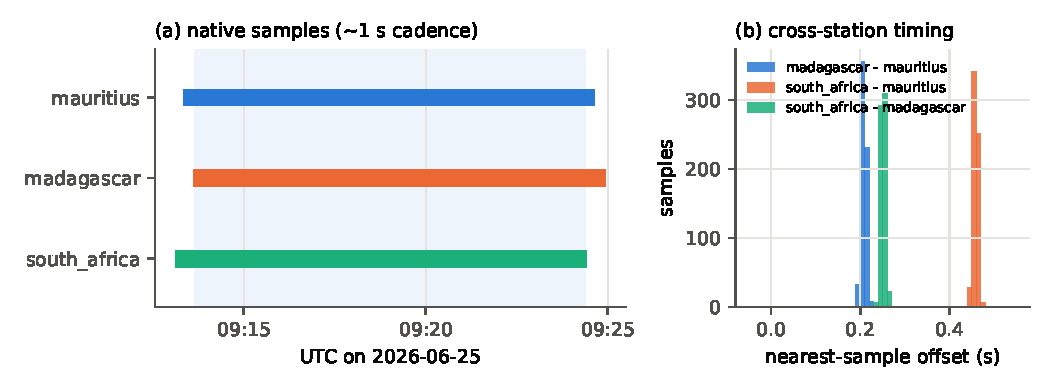
\includegraphics[width=\textwidth]{figures/stage2_timing.pdf}
\caption{Stage-2 real data, GPS BIIF-9 on 2026-06-25. (a)~Native samples
at each station (ticks merge at this scale) and the actual three-station
overlap (shaded). (b)~Offsets between each sample and the other station's
nearest sample, for each station pair: the dumps are offset by
0.2--0.5~s.}
\label{fig:stage2}
\end{figure}

%======================================================================
\part{Interfaces, limitations and reproducibility}
%======================================================================

\section{Interface to later stages}
\label{sec:future}

\paragraph{Stage 3 (imaging).} Stage~3 will need only the Stage-2 manifest,
\code{image-tart --manifest data/observations/20260625/NORAD\_40534/manifest.json}.
For each station the manifest gives the MS path, the actual sample times,
the calibration status and flagged fraction, and the Stage-1 predicted
azimuth and elevation. The synchronisation section gives the common
interval and the cross-station timing statistics needed to choose matching
epochs. A dataset with \code{three\_station\_valid=false} must not be used
for three-station localisation.

\paragraph{Stage 5 (inference).} For a candidate satellite position
$\vect r_s$ in ITRS, the predicted direction at station $i$ is
$\hat{\vect d}_i(\vect r_s)$, converted to $(A_i,E_i)$ in the local
east-north-up frame. Given TART-measured directions
$(A_i^{\rm obs},E_i^{\rm obs})$ with uncertainties $\sigma_i$, a natural
likelihood is
\begin{equation}
\ln\mathcal L(\vect r_s) = -\frac12\sum_{i=1}^{3}
\frac{\theta_i^2(\vect r_s)}{\sigma_i^2} + \text{const},\qquad
\cos\theta_i = \hat{\vect d}_i(\vect r_s)\cdot\hat{\vect u}_i^{\rm obs},
\end{equation}
where $\theta_i$ is the angle between predicted and observed unit vectors.
Stage~1 already provides every ingredient of the forward model --- exact
station ITRS vectors, exact UTC epochs, TLE provenance, predicted
$(A_i,E_i)$, predicted $\vect r_s$ and line-of-sight unit vectors --- and the
verification of Section~\ref{sec:verification} shows the angular and
Cartesian predictions are consistent to better than \ang{0.001}. A
TLE-based prior on $\vect r_s$ (or its comparison in Stage~6) should account
for the TLE age recorded with each window.

%======================================================================
\section{Limitations}
%======================================================================

\begin{itemize}
\item TLE/SGP4 accuracy depends on TLE age and quality; current CelesTrak
data are not suitable for reconstructing old observations
(Sections~3.3 and~7).
\item Visibility uses geometric elevation; refraction, local horizon masks
and antenna patterns are not modelled.
\item ITRS positions neglect polar motion ($\sim$\SI{10}{\metre}).
\item Station coordinates are as published by TART, with undocumented
accuracy and height datum. The registry schema is external and may change.
The parser then fails explicitly, and the frozen catalogue remains usable.
\item Registry presence does not mean a station is online or has archived
data. The registry's \code{online} flag is not used, and archive presence
is verified only at the prefix level, not for a particular date.
\item Excursions shorter than the coarse step are not detected.
\item Stage~1 does not filter satellites by transmitted signal. Stage~2
labels each window with \code{signal\_relevance}, but does not check
whether individual satellites are healthy.
\item Stage~2 relies on the archive's filename convention (verified on real
files) only to \emph{find} candidate files. All times used come from the
file contents.
\item Gain and phase solutions are applied as recorded and are not
verified. Station dumps are not simultaneous ($\lesssim$\SI{0.5}{\second}
offsets), and no epoch-matching rule has been fixed yet.
\item Live TART APIs were not used. Archive availability depends on each
station uploading its data; for example, Mauritius has no data after
2026-06-26.
\end{itemize}

%======================================================================
\section{Reproducibility}
%======================================================================

A run is fully reproducible from its metadata file: the archived TLE file
(verified by SHA-256), the station catalogue (also hashed, together with the
SHA-256 and retrieval time of the registry snapshot it was built from), the
software versions and the full command line. Registry snapshots, like TLE
catalogues, are archived under \code{data/stations/} and never overwritten. Re-running with
\code{--tle-file data/tle/gnss\_2026-10-07T101156Z.tle} reproduces the
Stage-1 results in this report. Historical catalogues are never
overwritten. A Stage-2 manifest records the SHA-256 of the Stage-1 file and
of the station file, the archive identifiers, URLs and SHA-256 of every
native file, the exact \code{tart2ms} command and the software versions
(including \code{tart2ms}, \code{tart-tools}, python-casacore, \code{h5py}
and \code{minio}), so the dataset can be re-retrieved and checked.

\begin{thebibliography}{99}
\bibitem{tart} T.~Molteno et al., \emph{TART: The Transient Array Radio
Telescope}, \url{https://tart.elec.ac.nz}; source code
\url{https://github.com/tart-telescope}.
\bibitem{celestrak} T.~S.~Kelso, \emph{CelesTrak GP element sets},
\url{https://celestrak.org/NORAD/elements/}.
\bibitem{skyfield} B.~Rhodes, \emph{Skyfield: High precision research-grade
positions for planets and Earth satellites generator}, Astrophysics Source
Code Library ascl:1907.024 (2019), \url{https://rhodesmill.org/skyfield/}.
\bibitem{sgp4} B.~Rhodes, \emph{sgp4: Python implementation of the SGP4
satellite propagation model}, \url{https://pypi.org/project/sgp4/}.
\bibitem{vallado2006} D.~A.~Vallado, P.~Crawford, R.~Hujsak and T.~S.~Kelso,
``Revisiting Spacetrack Report \#3,'' AIAA 2006-6753 (2006).
\bibitem{tart2ms} T.~Molteno, B.~Hugo et al., \emph{tart2ms: convert TART
observations to Measurement Sets}, \url{https://github.com/tart-telescope/tart2ms}
(v0.9.4).
\bibitem{tarttools} T.~Molteno et al., \emph{tart\_tools} (archive client
\code{tart\_tools.archive\_handler}), \url{https://pypi.org/project/tart-tools/} (v1.4.6).
\bibitem{gnssbook} P.~J.~G.~Teunissen and O.~Montenbruck (eds.),
\emph{Springer Handbook of Global Navigation Satellite Systems}, Springer (2017).
\end{thebibliography}

\appendix
\section{CSV columns}
\small
\code{rank, satellite\_name, norad\_id, constellation, common\_start\_utc,
common\_end\_utc, duration\_seconds, duration\_minutes, start\_clipped,
end\_clipped, min\_elevation\_deg}, then for $i=1,2,3$:
\code{station\_$i$, station\_$i$\_az\_\{start,mid,end\}\_deg,
station\_$i$\_el\_\{start,mid,end\}\_deg, station\_$i$\_range\_mid\_km}, then
\code{mid\_utc, coordinate\_frame, sat\_x\_mid\_km, sat\_y\_mid\_km,
sat\_z\_mid\_km, tle\_epoch, tle\_age\_start\_days, tle\_age\_mid\_days,
tle\_source}.

\end{document}
